

\begin{table}[ht!]
	\centering
	\small
	\begin{tabular}{p{2cm}p{2cm}p{2cm}p{5cm}p{1cm}} 
		\toprule
		\textbf{Operation} & \textbf{Matrix} & \textbf{Graph} & \textbf{Logic} & \textbf{Size} \\
		\midrule
		Initial 
		&
		$
		\begin{array}{c|c}
			& x  \\
			\hline
			y & 1 
		\end{array}
		$
		&
		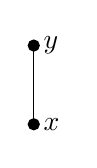
\begin{tikzpicture}[baseline=(current bounding box.center)]
			\draw[fill=black] (0,0) circle (2pt);
			\draw[fill=black] (0,1) circle (2pt);
			
			\draw (0,0) -- (0,1);
			
			\node[right] at (0,0) {$x$};
			\node[right] at (0,1) {$y$};
		\end{tikzpicture}
		&
		$\alpha(x,y)$		&3
		\\[2em]
Label
		&
		$
		\begin{array}{c|c}
			& H \\
			\hline
			y & 1 \\
		\end{array}
		$
		&
		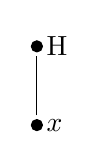
\begin{tikzpicture}[baseline=(current bounding box.center)]
			\node (x) at (0,0) {};
			\node (y) at (0,1) {};
			\draw[fill=black] (x) circle (2pt);
			\draw[fill=black] (y) circle (2pt);
			\draw (x) -- (y);
			\node[right] at (x) {$x$};
			\node[right] at (y) {H};
		\end{tikzpicture}
		&
		$		\alpha(x,y) \land H(x)$&3
		\\[2em]
Nodes
		&
		$\begin{array}{c|cc}
			& x & z \\
			\hline
			y & 1 & 
		\end{array}$		&
		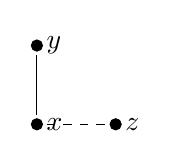
\begin{tikzpicture}[baseline=(current bounding box.center)]
			\node (x) at (0,0) {};
			\node (y) at (0,1) {};
			\node (z) at (1,0) {};
			
			\draw[fill=black] (x) circle (2pt);
			\draw[fill=black] (y) circle (2pt);
			\draw[fill=black] (z) circle (2pt);
			
			\draw (x) -- (y);
			\draw[dashed] (x) -- (z);
			
			\node[right] at (x) {$x$};
			\node[right] at (y) {$y$};
			\node[right] at (z) {$z$};
		\end{tikzpicture}
		&
		$
		\alpha(x,y) \land \exists z \lhd(x,z)$&4
		\\[2em]
		
		Association
		&
		$
		\begin{array}{c|cc}
			& x & z \\
			\hline
			y & 1 & 1
		\end{array}
		$
		&
		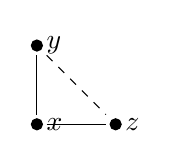
\begin{tikzpicture}[baseline=(current bounding box.center)]
			\node (x) at (0,0) {};
			\node (y) at (0,1) {};
			\node (z) at (1,0) {};
			
			\draw[fill=black] (x) circle (2pt);
			\draw[fill=black] (y) circle (2pt);
			\draw[fill=black] (z) circle (2pt);
			
			\draw (x) -- (y);
			\draw (x) -- (z);
			\draw[dashed] (y) -- (z);			
			\node[right] at (x) {$x$};
			\node[right] at (y) {$y$};
			\node[right] at (z) {$z$};
		\end{tikzpicture}
		&
		$		\alpha(x,y) \land \exists z\,\big(\lhd(x,z) \land \alpha(y,z)\, \big)$&5
		\\[2em]
	
		\bottomrule
	\end{tabular}
	
	\caption{Examples of operations used in generating 
		\textsc{NextSupFact} hypotheses across matrix, graph, and logical 
		representations. }
	\label{tab:nextsupfact}
\end{table}